The main complain about patent search is insufficient match between the content of patent queries and relevant
patents\cite{lupu2013patent}\cite{magdy2012toward}. However, we have the intuition that there are sufficient terms in a patent query containing thousands words to be matched with the relevant patents. So, in this section, we focused on term analysis to figure out the main causes that the system fails in retrieving relevant documents at top of the result list. 
\subsection{Oracular Query Formulation}
We started with {\em relevance feedback}, in which the user gives feedback on the relevance of documents in an initial set of results to improve the final result set. We calculate a relevance feedback (RF) score for each term in top-100 retrieved documents as follows:
\begin{equation}
score_{RF}(t,Q)=Rel(t)-Irr(t) 
 \label{eq:score}
\end{equation}\vspace*{-5ex}
\begin{displaymath}t\in \lbrace \mbox{terms in top-100 retrieved documents}\rbrace\end{displaymath}
where $ Rel(t) $ is the average term frequency in retrieved relevant patents and $ Irr(t) $ is the average term frequency in retrieved irrelevant patents. We assumed that words with a positive score are {\em useful words} since they are more frequent in relevant patents, while words with negative score are {\em noisy words} as they appear more frequently in irrelevant patents. 

We expected to see a higher performance for the queries which contain more {\em useful words}, but, surprisingly, we could not find any correlation between the performance and the percentage of {\em useful words} in the query. 

We hypothesized that a query, formulated by only the {\em useful terms}, is the best possible query we can make since they are all frequent in relevant patents but rare in irrelevant ones. We formulated an oracular query as follows: 
\begin{equation}
Oracular \; Query = \{t \in top-100|score_{RF}(t)>0\}   
 \label{eq:score}
\end{equation}

Our previous experiments led us to the hypothesis that a patent query contains sufficient words matched with the relevant patents.
% and the {\em noisy words} are the main cause of the low effectiveness. 
To prove our idea, we formulated a query by selecting only {\em useful terms} existing inside the patent query as follows: 
\begin{equation}
 Oracular \; Patent \; Query = \{t\in Q|score_{RF}(t)>0\}   
 \label{eq:score}
\end{equation}
The results were encouraging, as MAP was improved from 0.1181 to {\em 0.44}.
\subsection{Baseline vs. Oracular Query}
Table \ref{tab:optquery} compares the baseline performance, where the query is the full patent application, with the performance of the Oracular Query. 
\begin{table}[htpb]
  \begin{center}
   \caption{System performance for the baseline and ideal query.}
  \input table/optquery.tex   
  \label{tab:optquery}
  \end{center}  
\end{table}
It can be seen that MAP jumps from 0.1181 to {\em 0.5075}, which means the Oracular Query far outperforms the baseline and performs twice as well on MAP as the best competitor in CLEF-IP 2010~\cite{lopez2010experiments}. 

Figure \ref{fig:oracular} compares the result for Oracular Query and Oracular Patent Query, when we use a threshold $\tau$ for selecting terms to formulate a query. 
\begin{figure}[htpb]
   \centering
   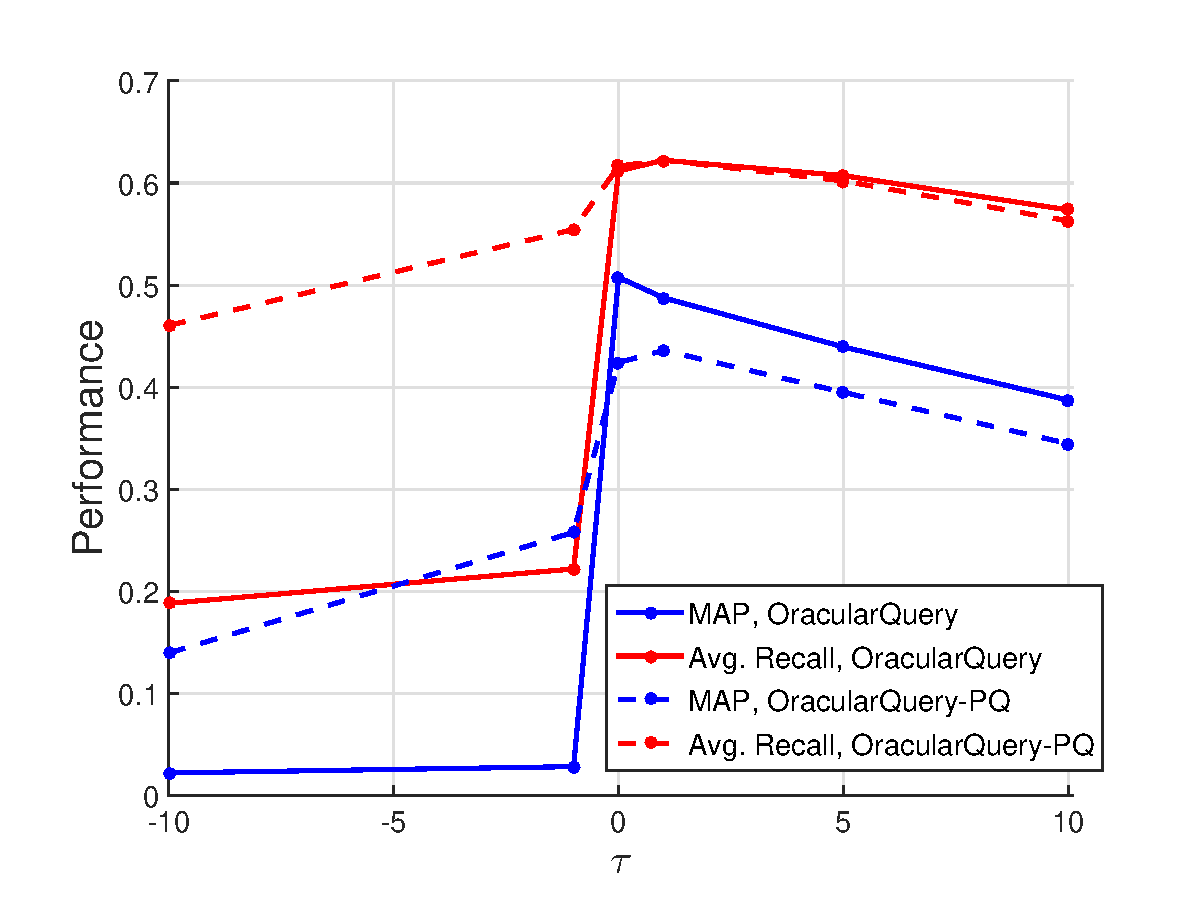
\includegraphics[width=0.30\textwidth,height=40mm]{figs/oracularquery.eps}
   \caption{System performance vs. the threshold $\tau$ for oracular query and oracular patent query.}   
   \label{fig:oracular} 
\end{figure} 
There two important fact in Figure \ref{fig:oracular} : (1) noisy terms ($\tau <0 $) can highly ruin the IR effectiveness. (2) a patent query contains sufficient useful terms to achieve an acceptable performance. Therefore, to improve patent prior-art search, we need to reformulate the initial patent query using term selection, and query reduction rather than query expansion. In addition, it is very important to identify and prune all the noisy words out because they are highly harmful.  